\documentclass[letter,11pt]{article}

\usepackage[spanish,es-nodecimaldot]{babel}
\usepackage[utf8]{inputenc}

\usepackage{lmodern}
\usepackage[T1]{fontenc}
\usepackage{textcomp}

\usepackage{framed}
\usepackage[svgnames]{xcolor}
\colorlet{shadecolor}{Gainsboro!50}

\usepackage{graphicx}
\usepackage{pstricks}

\usepackage{anysize}
\marginsize{3cm}{2cm}{2cm}{3cm}

\usepackage{amsmath}
\usepackage{array}
\usepackage{alltt}

\usepackage{fancyhdr}
\usepackage{lastpage}
\pagestyle{fancy}
\fancyhf{}
\fancyhead[LE,RO]{Laboratorio de Física Básica I}
\fancyfoot[CO,CE]{\thepage\ de \pageref{LastPage}}

\special{papersize=215.9mm,279.4mm}

\usepackage[
    pdfauthor={Carlos Eduardo Caballero Burgoa},%
    pdftitle={Laboratorio de Física Básica I},%
    pdfsubject={2do Parcial},%
    colorlinks,%
    citecolor=black,%
    filecolor=black,%
    linkcolor=black,%
    urlcolor=black,
    breaklinks]{hyperref}
\usepackage{breakurl}

\newcommand{\blankpage}{
\newpage
\thispagestyle{empty}
\mbox{}
\newpage
}

\renewcommand{\arraystretch}{1.2}

\begin{document}

\begin{center}
    {\Large \bf{Segundo parcial}}
\end{center}

\noindent\fbox{%
    \parbox{\textwidth}{%
        Estudiante: CABALLERO BURGOA, Carlos Eduardo \\
        Carrera: Ingeniería Electromecánica \\
        Correo: cijkb.j@gmail.com
    }%
}

\vspace{1.0cm}

\begin{enumerate}
\item La tabla a continuación presenta datos de posición en función del tiempo.
    Indique a que clase de movimiento corresponde, graficar y encuentre la
    ecuación empírica con su respectivo error.

    \begin{center}
    \begin{tabular}{|c|>{\centering}m{2.8cm}<{\centering}
                      |>{\centering}m{2.8cm}<{\centering}|}
    \hline
    $i$ & $t_i [s]$ & $x_i [m]$ \tabularnewline \hline
      1 & 0.0 &  3.00 \tabularnewline \hline
      2 & 0.2 &  4.62 \tabularnewline \hline
      3 & 0.4 &  6.17 \tabularnewline \hline
      4 & 0.6 &  7.83 \tabularnewline \hline
      5 & 0.8 &  9.39 \tabularnewline \hline
      6 & 1.0 & 10.98 \tabularnewline \hline
    \end{tabular}
    \end{center}

    Solución:

    Se obtiene el siguiente gráfico:

    \begin{figure}[!h]
    \centering
    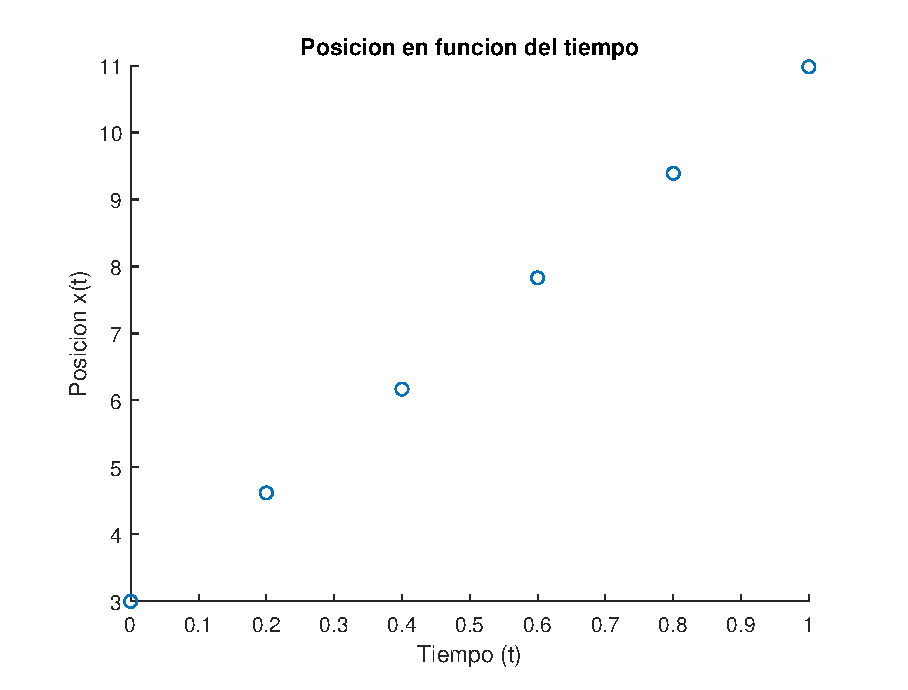
\includegraphics[scale=0.75]{resources/g1a.eps}
    \end{figure}

    Por tanto corresponde a un movimiento con $a = 0$, es decir
    \textbf{movimiento uniforme}.

    Calculando los valores de la recta por el método de los mínimos cuadrados,
    se obtiene:

    \begin{equation*}
        A = (3.00 \pm 0.02)[m];0.59\%
    \end{equation*}

    \begin{equation*}
        B = (7.98 \pm 0.03)[m/s];0.37\%
    \end{equation*}

    Con los parámetros obtenidos la relación $x = x(t)$ es:

    \begin{equation}
        x = 3 + 7.98 t
    \end{equation}

    \vspace{1.0cm}
    \textbf{Memoria de calculo:}
    \begin{shaded}
        \begin{alltt}
            \footnotesize
\# Datos importados (i1.csv):
\input{resources/i1.csv}

\# Comandos ejecutados (p1b.m):
\input{resources/p1b.m}

\# Salida del programa (o1b.txt):
\input{resources/o1b.txt}
            \normalsize
        \end{alltt}
    \end{shaded}

\newpage
\item La tabla a continuación presenta datos de posición en función del tiempo.
    Indique a que clase de movimiento corresponde, graficar y encuentre la
    ecuación empírica con su respectivo error.

    \begin{center}
    \begin{tabular}{|c|>{\centering}m{2.8cm}<{\centering}
                      |>{\centering}m{2.8cm}<{\centering}|}
    \hline
    $i$ & $t_i [s]$ & $x_i [m]$ \tabularnewline \hline
      1 & 0.0 & 0.000 \tabularnewline \hline
      2 & 0.1 & 0.009 \tabularnewline \hline
      3 & 0.2 & 0.038 \tabularnewline \hline
      4 & 0.3 & 0.091 \tabularnewline \hline
      5 & 0.4 & 0.164 \tabularnewline \hline
      6 & 0.5 & 0.251 \tabularnewline \hline
    \end{tabular}
    \end{center}

    Solución:

    Se obtiene el siguiente gráfico:

    \begin{figure}[!h]
    \centering
    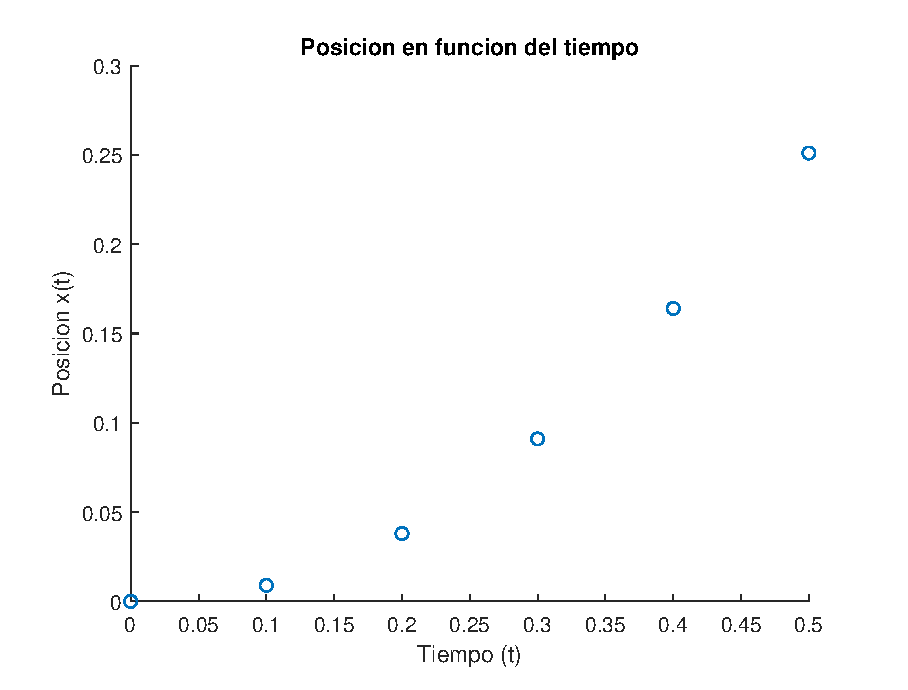
\includegraphics[scale=0.75]{resources/g2a.eps}
    \end{figure}

    Por tanto corresponde a un movimiento con $a \neq 0$, es decir
    \textbf{movimiento uniformemente acelerado}.

    Aplicando linealización por logaritmos:

    \begin{center}
    \begin{tabular}{|c|>{\centering}m{2.8cm}<{\centering}
                      |>{\centering}m{2.8cm}<{\centering}|}
    \hline
    $i$ & $\log(x_i)$ & $\log(t_i)$ \tabularnewline \hline
      1 & -       & -       \tabularnewline \hline
      2 & -1.0000 & -2.0458 \tabularnewline \hline
      3 & -0.6990 & -1.4202 \tabularnewline \hline
      4 & -0.5229 & -1.0410 \tabularnewline \hline
      5 & -0.3979 & -0.7852 \tabularnewline \hline
      6 & -0.3010 & -0.6003 \tabularnewline \hline
    \end{tabular}
    \end{center}

    \begin{figure}[!h]
    \centering
    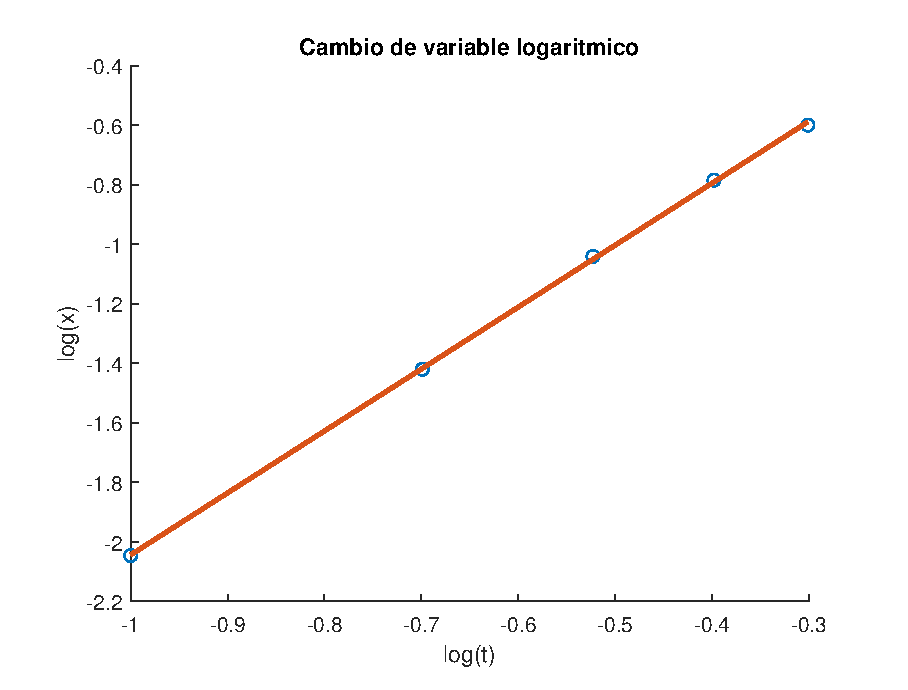
\includegraphics[scale=0.75]{resources/g2b.eps}
    \end{figure}

    \textbf{Memoria de calculo:}
    \begin{shaded}
        \begin{alltt}
            \footnotesize
\# Datos importados (i2.csv):
\input{resources/i2.csv}

\# Comandos ejecutados (p2b.m):
\input{resources/p2b.m}

\# Salida del programa (o2b.txt):
\input{resources/o2b.txt}
            \normalsize
        \end{alltt}
    \end{shaded}

    Calculando los valores de la recta por el método de los mínimos cuadrados,
    se obtiene:

    \begin{equation*}
        A = (0.03 \pm 0.01)[m];29.63\%
    \end{equation*}

    \begin{equation*}
        B = (2.08 \pm 0.02)[m/s];0.82\%
    \end{equation*}

    La ecuación de la recta es:

    \begin{equation*}
        Y' = 0.03 + 2.08 X'
    \end{equation*}

    A partir de los parámetros de recta $A$ y $B$, calculamos los parámetros $a$ y
    $b$, de la curva original y sus errores por el método de propagación de errores:

    \begin{equation*}
        a = antilog(A) = antilog(0.03) = 1.08
    \end{equation*}
    \begin{equation*}
        b = B = 2.08
    \end{equation*}
    \begin{equation*}
        e_a = 10^A ln(10) e_A = 10^{(0.03)} ln(10) 0.01 = 0.02
    \end{equation*}
    \begin{equation*}
        e_b = e_B = 0.02
    \end{equation*}

    Obteniendo finalmente los valores de la curva:

    \begin{equation*}
        a = (1.08 \pm 0.02)[m/s^2];2.49\%
    \end{equation*}

    \begin{equation*}
        b = (2.08 \pm 0.02)[u];0.82\%
    \end{equation*}

    La ecuación de la curva resultante es:

    \begin{equation}
        x = 1.08 t^2
    \end{equation}

    \textbf{Memoria de calculo:}
    \begin{shaded}
        \begin{alltt}
            \footnotesize
\# Datos importados (i2.csv):
\input{resources/i2.csv}

\# Comandos ejecutados (p2c.m):
\input{resources/p2c.m}

\# Salida del programa (o2c.txt):
\input{resources/o2c.txt}
            \normalsize
        \end{alltt}
    \end{shaded}

\newpage
\item La tabla presenta datos de aceleración ($a^*$) en función de la fuerza
    ($F$) para una práctica de dinámica. Determine la ecuación empírica
    aplicando MMC. Obtenga además el valor de la fuerza con su respectivo error.

    \begin{center}
    \begin{tabular}{|c|>{\centering}m{2.8cm}<{\centering}
                      |>{\centering}m{2.8cm}<{\centering}|}
    \hline
    $i$ & $F_i [s]$ & $a^*_i [m]$ \tabularnewline \hline
      1 & 0.49 & 99.92 \tabularnewline \hline
      2 & 0.98 & 50.14 \tabularnewline \hline
      3 & 1.96 & 25.85 \tabularnewline \hline
      4 & 4.90 &  9.96 \tabularnewline \hline
      5 & 9.80 &  4.82 \tabularnewline \hline
    \end{tabular}
    \end{center}

    Solución:

    Se obtiene el siguiente gráfico:

    \begin{figure}[!h]
    \centering
    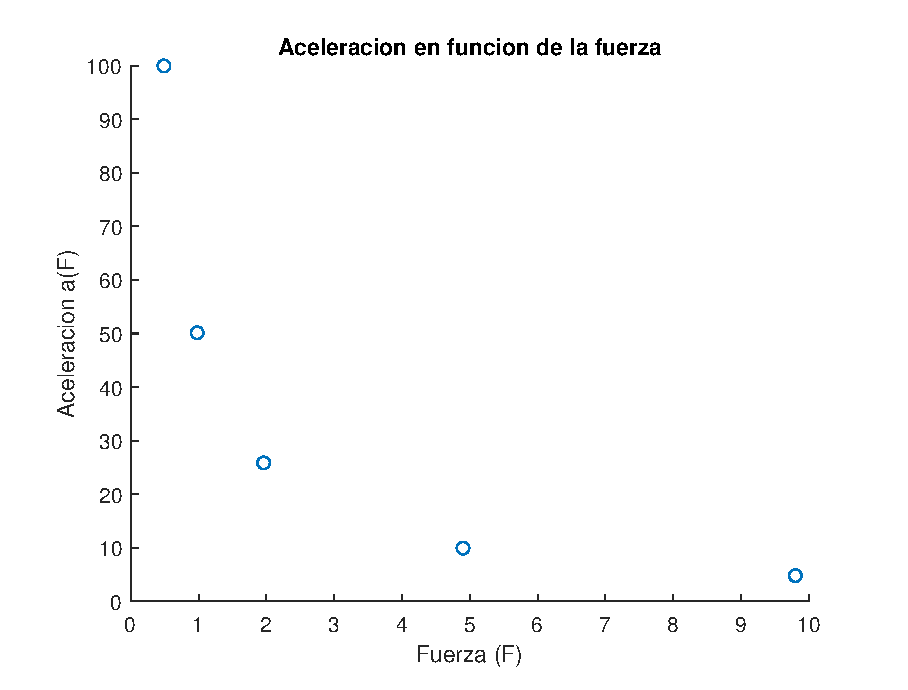
\includegraphics[scale=0.75]{resources/g3a.eps}
    \end{figure}

    Por lo tanto la relación entre fuerza ($F$) y aceleración ($a$), es
    inversamente proporcional.

    \begin{equation*}
        a \propto \frac{1}{F}
    \end{equation*}

    Aplicando linealización por logaritmos:

    \begin{center}
    \begin{tabular}{|c|>{\centering}m{2.8cm}<{\centering}
                      |>{\centering}m{2.8cm}<{\centering}|}
    \hline
    $i$ & $\log(F_i)$ & $\log(a_i)$ \tabularnewline \hline
      1 & -0.3098 & 1.9997 \tabularnewline \hline
      2 & -0.0088 & 1.7002 \tabularnewline \hline
      3 &  0.2923 & 1.4125 \tabularnewline \hline
      4 &  0.6902 & 0.9983 \tabularnewline \hline
      5 &  0.9912 & 0.6830 \tabularnewline \hline
    \end{tabular}
    \end{center}

    \begin{figure}[!h]
    \centering
    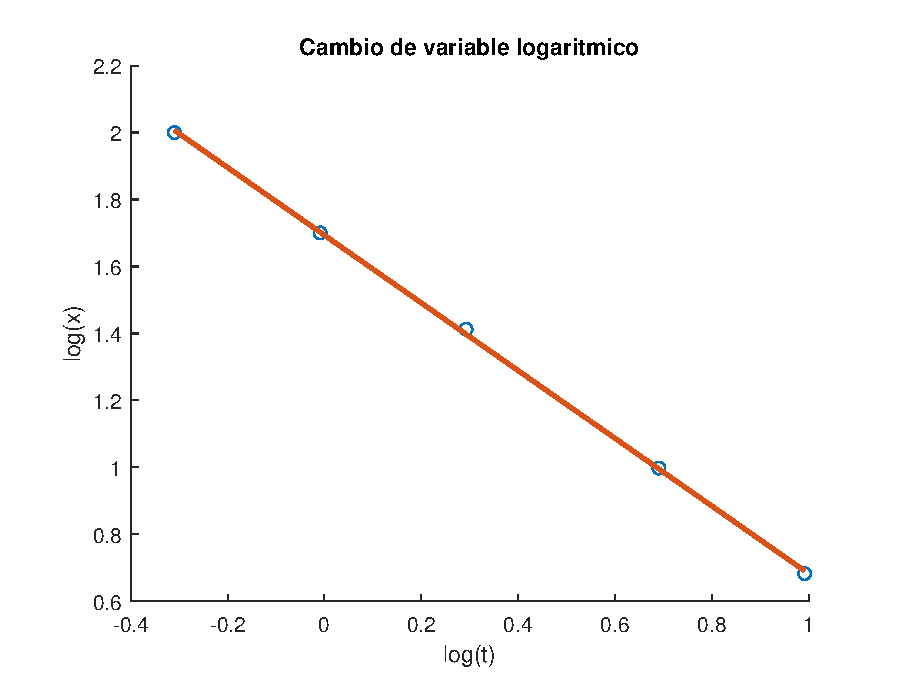
\includegraphics[scale=0.75]{resources/g3b.eps}
    \end{figure}

    \textbf{Memoria de calculo:}
    \begin{shaded}
        \begin{alltt}
            \footnotesize
\# Datos importados (i3.csv):
\input{resources/i3.csv}

\# Comandos ejecutados (p3b.m):
\input{resources/p3b.m}

\# Salida del programa (o3b.txt):
\input{resources/o3b.txt}
            \normalsize
        \end{alltt}
    \end{shaded}

    Calculando los valores de la recta por el método de los mínimos cuadrados,
    se obtiene:

    \begin{equation*}
        A = (1.69 \pm 0.006)[m];0.34\%
    \end{equation*}

    \begin{equation*}
        B = (-1.01 \pm 0.01)[m/s];1.00\%
    \end{equation*}

    La ecuación de la recta es:

    \begin{equation*}
        Y' = 1.69 - 1.01 X'
    \end{equation*}

    A partir de los parámetros de recta $A$ y $B$, calculamos los parámetros $a$ y
    $b$, de la curva original y sus errores por el método de propagación de errores:

    \begin{equation*}
        a = antilog(A) = antilog(1.68) = 49.36
    \end{equation*}
    \begin{equation*}
        b = B = -1.01
    \end{equation*}
    \begin{equation*}
        e_a = 10^A ln(10) e_A = 10^{(1.69)} ln(10) 0.006 = 0.66
    \end{equation*}
    \begin{equation*}
        e_b = e_B = 0.01
    \end{equation*}

    Obteniendo finalmente los valores de la curva:

    \begin{equation*}
        a = (49.36 \pm 0.66)[u];1.34\%
    \end{equation*}

    \begin{equation*}
        b = (-1.01 \pm 0.01)[u];1.00\%
    \end{equation*}

    La ecuación de la curva resultante es:

    \begin{equation}
        a = \frac{49.36}{F}
    \end{equation}

    \textbf{Memoria de calculo:}
    \begin{shaded}
        \begin{alltt}
            \footnotesize
\# Datos importados (i3.csv):
\input{resources/i3.csv}

\# Comandos ejecutados (p3c.m):
\input{resources/p3c.m}

\# Salida del programa (o3c.txt):
\input{resources/o3c.txt}
            \normalsize
        \end{alltt}
    \end{shaded}

\end{enumerate}
\end{document}

